\documentclass{article}

% preambulo:
\input{Control_tp3_preamble.tex}

\usepackage{fancyhdr}

\geometry{top=2.5cm, bottom=2.0cm, left=2.25cm, right=2.25cm}

\lhead{Sistemas de Control 22.85}
\chead{TP3 - Control Servo}
\rhead{ITBA}
\renewcommand{\headrulewidth}{1pt}
\renewcommand{\footrulewidth}{1pt}
\pagestyle{fancy}


\begin{document}

%\newgeometry{} % margenes default para la caratula
% caratula:
\input{Control_tp3_caratula.tex}


% indice:
\tableofcontents
\newpage

\section{Análisis del Motor de CC}

En primer lugar se considera el modelo circuital para el motor utilizado, teniendo en cuenta que los diferentes parámetros son datos provistos por la hoja de datos del QUANSER:

\begin{figure}[H]
\centering
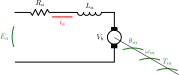
\includegraphics[width=0.5\linewidth]{../Images/ModeloMotor.png}
\end{figure}

Las ecuaciones que caracterizan al sistema son:

\[
\left\lbrace
\begin{array}{ll}
E_a = R_a \cdot i_a + L_a \cdot \dot{i_a} + V_b \\
V_b = K_b \cdot \omega_m = K_b \cdot \dot{\theta_m} \\
T_m = J_m \cdot \ddot{\theta_m} + B_m \cdot \dot{\theta_m} + T_l
\end{array}
\right.
\]

De las cuales se puede obtener las funciones de transferencia de $\theta_l$ y $\omega_m$ respecto a la tensión de alimentación $E_a$:

\[
\frac{\omega_m}{E_a} = \frac{\frac{K_t}{R_a \cdot J_m}}{S + \frac{B_m}{J_m} + \frac{K_t \cdot K_b}{R_a \cdot J_m}}
\]

\[
\frac{\theta_m}{E_a} = \frac{\frac{K_t}{R_a \cdot J_m}}{S \cdot (S + \frac{B_m}{J_m} + \frac{K_t \cdot K_b}{R_a \cdot J_m})}
\]

\end{document}
